\section{Rayman}

\begin{figure}[htbp]
\begin{center}
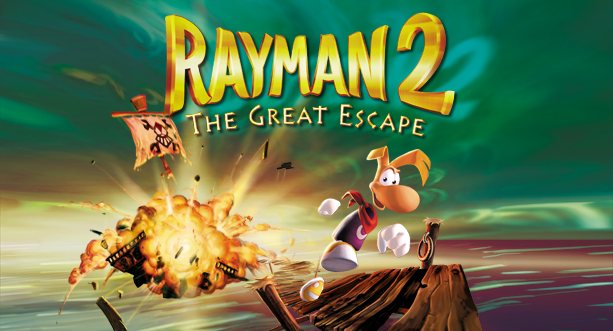
\includegraphics[width=.60\textwidth]{./imagenes/rayman.jpg}
\caption{Rayman}
\label{Rayman}
\end{center}
\end{figure}
Rayman\footnote{\url{http://www.onlinemania.org/juego/11605/Rayman-2--The-Great-Escape-8PSX9.html}} es un juego de aventura donde eres un personaje que debe salvar al mundo de unos malvados piratas roboticos venidos del espacio en naves espaciales con forma de barcos de guerra  gigantescos han invadido el planeta y, capturado y encerrado a la mayoria de sus habitantes. 
Rayman es apresado pero luego logra escapar para buscar Las Cuatro Máscaras, liberando a todo sus amigos, recogiendo los lums de energia y derrotar a los piratas. 
En la figura \ref{Rayman} puede ver una implementación del juego.
La premisa del juego: Recoger los lums de energia y las Cuatro Máscaras.

\subsubsection{¿Por qué es uno de mis juegos favoritos?}
\begin{itemize}
\item[Manuel Suárez] El juego que se me hizo mas fácil jugar, ademas Rayman es un personaje amigable y muy interesante. 
Se basa en un mundo mitico donde los seres son de diferentes razas pero que se apoyan para lograr tener o establecer un estado de paz entre las naciones
este se ve alterado por enemigos que buscan distorsionar este estado y lograr cometer barbaridades. 


\end{itemize}
